
%%% Local Variables: 
%%% mode: latex
%%% TeX-master: t
%%% End: 

\documentclass[UTF8]{ctexart}

\usepackage{latexsym}
\usepackage{amsmath}
\usepackage{amssymb}
\usepackage{graphicx}
\usepackage{wrapfig}
\usepackage{fancyhdr}
\usepackage{setspace}
\usepackage{framed}
\usepackage{hyperref}
\usepackage[table]{xcolor}
\definecolor{shadecolor}{rgb}{0.92,0.92,0.92}

\begin{document}

% 页眉 页脚 封面 定义

%%% Local Variables: 
%%% mode: latex
%%% TeX-master: "russian"
%%% End: 

\newcommand{\HRule}{\rule{\linewidth}{0.5mm}}
\newenvironment{shell}{\footnotesize{}\linespread{0.9}\begin{shaded}}{\end{shaded}\linespread{1.0}\normalsize{}}

% 首行缩进设置
\setlength{\parindent}{2em}
% 中文标题
\CTEXsetup[number={\chinese{section}}]{section}
\setlength{\fboxrule}{1pt}
\setlength{\fboxsep}{5pt}

% 页眉 页脚
\pagestyle{fancy}
\lfoot{FSF 2012} 
\cfoot{the machine of awareness}
\rfoot{\thepage} 
\renewcommand{\headrulewidth}{0.4pt} 
\renewcommand{\footrulewidth}{0.4pt}

\begin{titlepage}
  \begin{center}
    % Upper part of the page
    \includegraphics[width=2in]{images/gnu-head}
    \textsc{\LARGE }\\[1.5cm]
    \textsc{\Large 觉知的机器}\\[0.5cm]

    % Title
    \HRule \\[0.4cm]
    {\LARGE \bfseries GTK+2.0俄罗斯方块游戏设计v1.1}\\[0.4cm]
    \HRule \\[1.0cm]
    \textsc{\large Life is real only then, when ``I am''\\
      \quad{}G.I.GURDJIEFF}\\[2.0cm]

    % Author and supervisor
    \begin{minipage}{0.4\textwidth}
      \begin{center} \large
        编\quad{}写:\\
        觉知的机器
      \end{center}
    \end{minipage}

    \vfill
    % Bottom of the page
    {\large 甘肃兰州安宁机器工作室}\\ 
    {\large 2012年10月07日}
  \end{center}
\end{titlepage}



% 生成目录
\tableofcontents
\newpage

\begin{abstract}
  作者用Gtk+2.0编写了俄罗斯方块游戏,作为Gtk+2.0学习的练习,在这里将心得写出来和
  大家分享。游戏用方向键控制俄罗斯方块的移动与变换,当某行方块全满,自动清除,游
  戏只是个示例,没有计分系统。

  俄罗斯方块程序写了两个版本,一个版本使用程序写界面,一个版本使用glade设计界面,相
  比较用glade的版本代码更少,设计更灵活。

  运行环境:Debian6.0,gtk+-2.20.1,编程环境:emacs23.2,gcc-4.4.5,make-3.81。
\end{abstract}

% 介绍

%%% Local Variables: 
%%% mode: latex
%%% TeX-master: "russian"
%%% End: 

\section{Gtk介绍}

GTK+最初是GIMP的专用开发库,后来发展为Unix-like系統下开发图形界面的应用程序的主流
开发工具之一。GTK+是自由软件,并且是GNU计划的一部分。GTK+的许可协议是LGPL。

最初,GTK+ 是作为另一个著名的开放源码项目 —— GNU Image Manipulation Program
(GIMP) —— 的副产品而创建的。在开发早期的 GIMP 版本时,Peter Mattis 和 Spencer
Kimball 创建了 GTK(它代表 GIMP Toolkit),作为 Motif\footnote{Motif 最初是
  由 OSF(开放基金协会)开发的一个工业标准的 GUI(图形用户接
  口)。1996年,OSF 与 X/Open 合并为 Open Group,1997年初,X 联盟结束,并将其归属
  的项目移交给 Open Group。Open Group 继续开发和支持X窗口系统,Motif,CDE,和其他
  技术。2000年5月15日,Open Group 使用公共许可证向开放源代码团体发布了 Motif 的源
  代码。在开放系统(如 Linux)上,可以使用免费的 Motif。} 工具包的替代,后者在那个
时候不是免费的。(当这个工具包获得了面向对象特性和可扩展性之后,才在名称后面加上
了一个加号。)

与其他很多部件工具箱不同,GTK+ 并不基于Xt\footnote{Xt Intrinsics又名Xt 或 X
  Toolkit, 是X Window 的函式庫。Intrinsics 首先提供物件導向的程式設計架構,並引進
  了「widget」的概念。Motif、OpenLook 和 Lesstif 等即以 Xt 為基礎。Athena
  Toolkit也是衍生自 Xt Library。但一些知名的工具箱如 FLTK, GTK, 和 Qt 並不使
  用 Xt library, 反是直接使用 Xlib.}。这一决策优劣互见:优点是GTK+可以应用于其他
系统,其灵活性也很强;而缺点就是它无法利用以传统方法为X11定制的X资源数据库。GTK+
最早應用於X Window System,如今已移植至其他平台,諸如Microsoft
Windows、DirectFB\footnote{DirectFB是一个轻量级的提供硬件图形加速,输入设备处理和
  抽象的图形库,它集成了支持半透明的视窗系统以及在LinuxFramebuffer驱动之上的多层
  显示。它是一个用软件封装当前硬件无法支持的图形算法来完成硬件加速的
  层。DirectFB是为嵌入式系统而设计。它是以最小的资源开销来实现最高的硬件加速性
  能。},以及Mac OS X的Quartz\footnote{Quartz是位於Mac OS X的Darwin核心之上的繪圖
  層,有時候也認為是CoreGraphics。Quartz直接地支援Aqua,藉由顯示2D繪圖圖形來建立
  使用者介面,包含即時繪製(rendering)和次像素(sub-pixel)精準的反鋸齒。}.

\subsection{为什么使用Gtk+2.0}

Gtk+是自由软件,意味着每个人不仅可以自由地获得和使用这个工具包,还可以在满足某些条
件的情况下修改并重新发布它。它得到了积极的开发与维护,围绕它有一个充满活力的社区。

GTK+ 是可移植的。这意味着用户可以在许多平台和系统上运行它。另一方面,开发人员可以
把软件提供给众多用户,却只要编写一次程序,还可以使用许多不同的编程和开发平台、工
具和编程语言。所有这些都可以理解为更多的潜在用户,您可以利用更好地满足需求的更广
泛的技能和工具。

GTK+ 是采用软件开发中的最新技术开发的,使用现代的软件意味着,您不会陷在过时的工作
中,而跟不上时代的发展。持续的维护和开发也意味着您拥有影响工具包的未来发展方向的
能力。

% 面向对象

%%% Local Variables: 
%%% mode: latex
%%% TeX-master: "russian"
%%% End: 

\section{Gtk编程特点}

\subsection{类型转换}

GTK+一般使用c语言来撰写,c语言不支持面向对象,但GTK使用一些方式,支持一点面向对象
概念。GTK以结构体(struct)模拟类(class);新建类用gtk\_xxx\_new(type)的方式;使 用函
数名区分毎组类的方法,与GtkWindow相关的方法,都以gtk\_window开 头,如要设
置window的标题,使用:

\begin{shell}
\begin{verbatim}
gtk_window_set_title(GTK_WINDOW(window), "awareness");
\end{verbatim}
\end{shell}

gtk\_window\_set\_title第一个参数接受GtkWindow指针,通过这种方式,一组公用方法就
专 属GtkWindow类使用了。GTK的类中只有数据,没有方法,调用相关方法要传递类指针;由
于没有多态概念,传入 的指针必须转换为指定类型,如GTK\_WINDOW,把指针转换
为GtkWindow类型,GTK\_WINDOW是一个宏,用来进行指针类型转换,定义如
下 gtkwindow.h(usr/include/gtk-2.0/gtk)中:

\begin{shell}
\begin{verbatim}
#define GTK_WINDOW(obj)                                                       
        (G_TYPE_CHECK_INSTANCE_CAST((obj), GTK_TYPE_WINDOW, GtkWindow))
\end{verbatim}
\end{shell}

G\_TYPE\_CHECK\_INSTANCE\_CAST宏定义在GLib的 gtype.h(usr/include/glib-2.0/gobject)中:

\begin{shell}
\begin{verbatim}
#define G_TYPE_CHECK_INSTANCE_CAST(instance, g_type, c_type)
    (_G_TYPE_CIC ((instance), (g_type), c_type)) 
\end{verbatim}
\end{shell}

G\_TYPE\_CHECK\_INSTANCE\_CAST宏会检查instance是否为g\_type的一个实例,如果不是 的话就
发出警示讯息,若是的话就将指标转型为c\_type型态。GTK实际上使用结构链接(link)的方
式,GTK中的类继承关系如下:

\begin{shell}
\begin{verbatim}
GObject                                                                       
 +--GInitiallyUnowned                                                         
     +-- GtkObject                                                            
           +-- GtkWidget                                                      
                 +-- GtkContainer                                             
                       +-- GtkBin                                             
                             +-- GtkWindow  
\end{verbatim}
\end{shell}

G\_TYPE\_CHECK\_INSTANCE\_CAST就是根据这继承关系作转换的,在GTK定义中,毎个高 层次的
类都会包含低层次类,如:

\begin{shell}
\begin{verbatim}
struct _GtkWindow
{
  GtkBin bin;

  gchar *GSEAL (title);
  gchar *GSEAL (wmclass_name);
  gchar *GSEAL (wmclass_class);
  gchar *GSEAL (wm_role);

  GtkWidget *GSEAL (focus_widget);
  GtkWidget *GSEAL (default_widget);
  GtkWindow *GSEAL (transient_parent);
  GtkWindowGeometryInfo *GSEAL (geometry_info);
  GdkWindow *GSEAL (frame);
  GtkWindowGroup *GSEAL (group);

  guint16 GSEAL (configure_request_count);
  guint GSEAL (allow_shrink) : 1;
  guint GSEAL (allow_grow) : 1;
  guint GSEAL (configure_notify_received) : 1;
  ...
}

struct _GtkContainer                                                          
{                                                                             
  GtkWidget widget;                                                           

  GtkWidget *focus_child;                                                     

  guint border_width : 16;                                                    

  /*< private >*/                                                             
  guint need_resize : 1;                                                      
  guint resize_mode : 2;                                                      
  guint reallocate_redraws : 1;                                               
  guint has_focus_chain : 1;                                                  
}; 
\end{verbatim}
\end{shell}

GtkWindow的成员有一个GtkBin,GtkContainer的成员中有一个GtkWidget。

\subsection{事件处理模式}

\subsubsection{事件和信号}

所有图形环境的事件都是从系统(Gnome)传递来的,Gtk当然也是这样,事件通常由用户输
入产生,如按键、鼠标,或控件焦点改变。当你按下鼠标键,系统(Gnome)就产生事件,并
放入事件队列中,系统根据鼠标点击的坐标确定是哪个GtkWidget对象产生的事件,如按下
的是button按钮,事件结构体包将含有坐标信息,产生事件的button指针。

事件分为event和signal,event来自GDK事件体系,GDK事件又来自于系统。信signal是二次
包装后添加到GTK中的,再次包装的原因是GDK事件不够健壮、灵活。本质上
说,event是Gdk/Xlib的概念,event是从系统传递来的信息流,event放入队列,在GTK主循
环中(main loop)处理。signal是GtkWidget的子类,当有鼠标按动时,并不产生信号,信
号只是记录与之相关的回调函数(callback),signal由GtkWidget对象发出,和GTK主循环
无关。总之,event产生于系统,用GDK传递到程序,signal由产生GtkWidget对象发出,比
如,用鼠标按下button按钮时,系统在button上产
生``button\_press\_event'',接着button发出``cilcked signal''。并不是所有事件都有
对应信号,如拖曳(drag\_event)就没有对应的signal;相应的,并不是所有signal都有对
应event ,GtkWidget对象能产生自己的signal。

\subsubsection{事件定义}

为了连结一个事件与Callback函数,一样是使用g\_signal\_connect(),不过处
理event的Callback函式与signal的Callback函式在宣告时有些不同,以下是Callback函数定
义:

\begin{shell}
\begin{verbatim}
// 处理event回调函数
gboolean callback_func(
          GtkWidget *widget, GdkEvent *event, gpointer callback_data);
// 处理signal回调函数
void callback_func(
          GtkWidget *widget,  gpointer callback_data);
\end{verbatim}
\end{shell}

处理event的Callback函数多了一个GdkEvent*参数,而返回值的部份,可以控制事件是否进行
下一步传播,传回TRUE表示这个事件到止已获得处理,事件不用继续传播,将不会发出对应
的signal,传回FALSE表示事件继续传播,GtkWidget对象发出对应的signal。

event的处理函数会在signal的处理函数之前先处理,以按下按钮为例,基本上的
顺序为:
\begin{shell}
\begin{verbatim}
按钮按下 --> 发出 button_press_event --> 预设处理函数
                 --> 发出 clicked signal --> 预设处理函数
\end{verbatim}
\end{shell}

您可以设置事件的Callback函数,拦截button\_press\_event,当处理完传回TRUE时,就不
会发出clicked的signal,也就不会继续预设的signal处理函数,只有在传回FALSE时,才会
发出clicked的signal,则设置的signal处理函数才会被执行。

% gtk绘图方式

%%% Local Variables: 
%%% mode: latex
%%% TeX-master: "russian"
%%% End: 

\section{Gtk绘图方式}

GtkWidget对象中,GtkDrawingArea是专门用于绘图的,不用设置它的GTK\_APP\_PAINTABLE
标记,它的默认expose\_event回调函数不绘制形状,不会覆盖你自己绘制的图形。

在Gtk中,可以在GtkWidget对象上绘图,但必须设置GTK\_APP\_PAINTABLE标记,否
则,当对象接收到对象默认的expose\_event事件,你绘的图会被覆盖,当对象发生
expose\_event事件时,事件传递过程是这样的:
\begin{itemize}
\item 自己定义的expose\_event回调函数运行,在函数里绘制需要的图形
\item 对象默认的expose\_event回调函数运行,如果对象的GTK\_APP\_PAINTABLE标记未
  置位,会在函数里绘制对象默记形状,你自己绘制的图形会被覆盖;如果对象
  的GTK\_APP\_PAINTABLE标记置位,函数不会在函数里绘制对象默记形状
\item 父类的expose\_event回调函数运行
\end{itemize}

绘图命令将图形绘制在GdkDrawable对象上,GdkDrawable是一个接口,支持绘制图
形,包括GdkWindow,GdkPixmap,GdkBitmap对象,GdkDrawable是GObject的子类。Gtk绘图
命令有:绘点、直线、弧线、多边形、文字、图片等。绘图的内容可以在GdkDrawable对象间
方便的复制,也可以在GdkImage、GdkPixbuf之间复制,这些使GdkDrawable成为功能强大的
对象。

所有的绘图方法操作GdkDrawable对象,并将GdkDrawable对象作为方法的第一个参数。由于
绘图中经常要指定绘图参数,如绘制的前景色、背景色、线宽等,GDK定义了GdkGC结构包含
这些信息,这样用一个GdkGC参数,就可以将各种参数传递给绘图方法。

\subsection{内存中绘图}

直接在GtkWidget上绘图是简单的,当expose\_event事件发生时就有麻烦了,你需要记住绘
制过的所有图形,然后在事件回调函数中重新绘制,这是很讨厌的。解决的办法是将图形绘
制在内存中,但并不显示,当需要显示到屏幕或有expose\_event事件发生时,从内存复制相应
的内容到GtkWidget对象中。我们直接操作的对象是GdkPixmap,是GdkDrawable的子
类,GdkPixmap是资源对象。

下面是生成GdkPixmap的方法,drawable参数是对应显示图形的GdkDrawable对象,一般
是GtkWidget对象的GdkWindow对象(widget$\rightarrow{}$window),显示到屏幕就是
把GdkPixmap中的内容复制到drawable中。depth表示绘图毎一点占位的大小,安全的方式是
置成-1,GdkPixmap会自动设制位的大小。

\begin{shell}
\begin{verbatim}
GdkPixmap* gdk_pixmap_new (GdkDrawable *drawable, // to determine depth of pixmap
                           gint width,            // width of pixmap in pixels
                           gint height,           // height of pixmap in pixels
                           gint depth);           // bits per pixel
\end{verbatim}
\end{shell}

当将GdkPixmap中的内容(图形)显示到屏幕上(GtkDrawingArea的GdkWindow),需要调
用gdk\_draw\_drawable方法,调用后,会自动将GdkPixmap内容复制到GdkWindow中。
xsrc,ysrc是源(GdkPixmap)的起始坐标,xdest,ydest是目标(GdkWindow)的起始地
址,width,height是复制区域大小,如果要复制整个区域,可以将width或height设成-1。

\begin{shell}
\begin{verbatim}
void gdk_draw_drawable (GdkDrawable *target_drawable,
                        GdkGC *gc,
                        GdkDrawable *src,
                        gint xsrc,
                        gint ysrc,
                        gint xdest,
                        gint ydest,
                        gint width,
                        gint height);
\end{verbatim}
\end{shell}

绘图的过程一般是这样的,先将图形绘制到GdkPixmap中,然后调
用gtk\_widget\_queue\_draw\_area方法,方法中指定需要重绘的区域,系统会将这个区域
置成invalidate状态,置invalidate状态会触发expose\_event,expose\_event回调函数参
数中有区域信息,调用gdk\_draw\_drawable方法,将GdkPixmap中指定区域复制
到GdkWindow的指定位置,图形就显示出来了。方法中的x,y是置成invalidate状态的区域起
始坐标,width,height是区域大小。

如果整个GdkDrawingArea被遮住又重新显示,系统会自动产生expose\_event事件,回调函数
参数有区域信息,就是GdkDrawingArea的全部区域。

\begin{shell}
\begin{verbatim}
void gtk_widget_queue_draw_area (GtkWidget *widget,
                                 gint x,
                                 gint y,
                                 gint width,
                                 gint height);
\end{verbatim}
\end{shell}

% russian算法

%%% Local Variables: 
%%% mode: latex
%%% TeX-master: "russian"
%%% End: 

\section{游戏的结构}


程序用Gtk的面向对象的方式设计,有三个类实现,Diamone是单方块类,实现了单方块的显
示、移动,Mass是形状类,实现了7种俄罗斯方块形状的显示、移动、转换,DataBase是数据
库类,实现所有数据存取、处理,主程序调用Mass类、DataBase类。


\begin{shell}
\begin{verbatim}                         
        +--------------+ 4               1+-------------+           
        |   Diamond    +o-----------------+     mass    +           
        +--------------+            +----o+-------------+           
       russian_diamond_leftmove     |  2  russian_mass_leftmove     
       russian_diamond_rightmove    |     russian_mass_rightmove    
       russian_diamond_downmove     |     russian_mass_downmove     
                                    |     russian_mass_translate    
                                    |                               
                        1           |                               
        Russian主函数---------------+                               
                                    |                               
                                    |       russian_db_init         
                                    |       russian_db_repair_matrix
                                    |   1   +-----------+
                                    +------o+ DataBase  +
                                            +-----------+
\end{verbatim}
\end{shell}


\subsection{主程序}


主程序中绘制程序界面,实现事件回调函数;在expose-event事件中调
用gdk\_draw\_drawable,把内存图形显示到绘图区域;在key-press-event事件中调
用Mass类的russian\_mass\_leftMove、russian\_mass\_rightMove等方法响应上下左右按键操
作;在定时事件中调用DataBase类和Mass类的方法,实现俄罗斯方块的定时下落。

主程序中界面由运行区、后备区、开始按键、暂停按键组成,方块毎隔500mS下落一行;程序
中用table布局,界面为左右结构左边是运行区,右边是后备区、开始按键、暂停按键,参
见\pageref{fig:russian}页图\ref{fig:russian};运行区显示的是当前的形状,后备
区中显示将要在运行的形状,如当前形状下落到底,后备形状就成为当前形状,后备区随机
生成一个后备形状;程序中后备区和开始按键放入GtkVBox控件中,用vbox和alignment实
现,右边控件紧缩在一起的效果,下面的一段程序:

\begin{figure}[htbp]
  \centering
  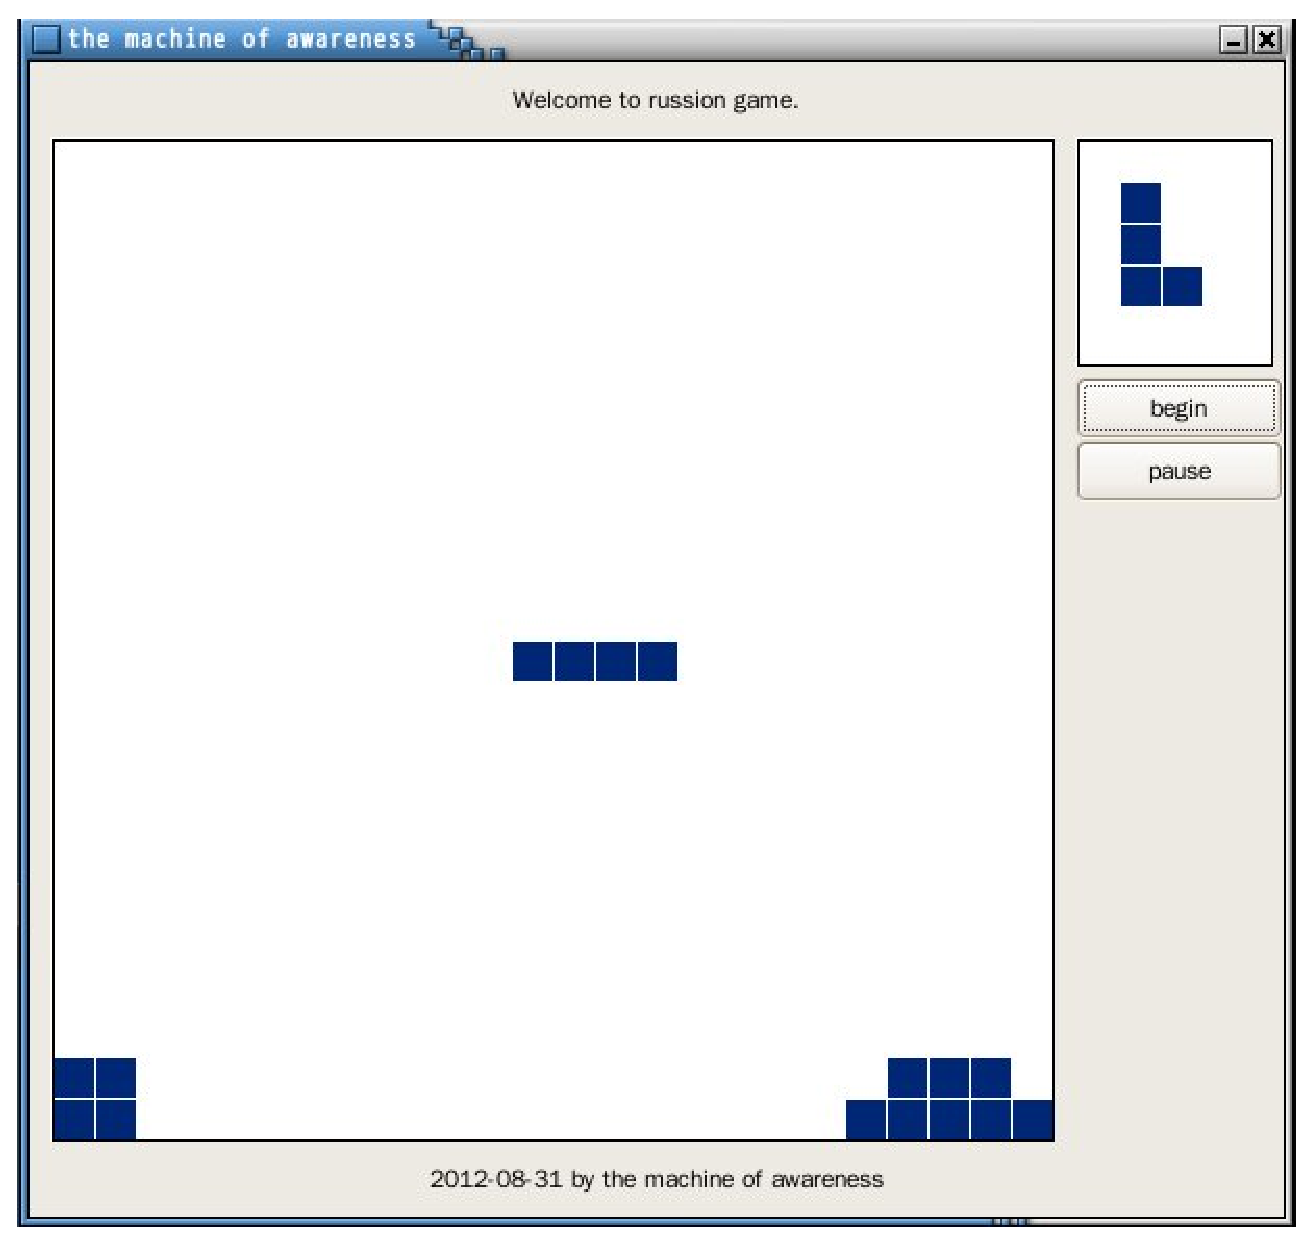
\includegraphics[width=3.5in]{images/russian}
  \caption{游戏界面}
  \label{fig:russian}
\end{figure}

\begin{shell}
\begin{verbatim}
  // 这里,用vbox和alignment实现,右边控件紧缩在一起的效果
  // vbox中包含的widget
  vbox = gtk_vbox_new(FALSE, 5);
  // s_drawArea
  // 设置s_drawArea的expose事件,在事件中显示图形
  g_signal_connect(s_drawArea, "expose-event", G_CALLBACK(on_s_expose), draw_info);
  // 实现右边控件紧缩在一起的效果,vbox的yoptions一定为要GTK_FILL
  gtk_table_attach(GTK_TABLE(table), vbox, 1, 2, 1, 2, 0, GTK_FILL, 0, 0);    
  gtk_widget_set_size_request(s_drawArea, 95, 110);
  gtk_box_pack_start(GTK_BOX(vbox), s_drawArea, FALSE, FALSE, 0);
  // button
  button = gtk_button_new_with_label("begin");
  g_signal_connect(button, "clicked", G_CALLBACK(on_begin), pause_button);
  gtk_widget_set_size_request(button, 100, 30);
  gtk_box_pack_start(GTK_BOX(vbox), button, FALSE, FALSE, 0);
  // alignment
  alignment = gtk_alignment_new(0, 0, 0, 0);
  gtk_widget_set_size_request(pause_button, 100, 30);
  gtk_container_add(GTK_CONTAINER(alignment), pause_button);
  // 实现右边控件紧缩在一起的效果,alignment的yoptions一定为要GTK_FILL|GTK_EXPAND
  gtk_table_attach(GTK_TABLE(table), alignment, 1, 2, 2, 3, 0, GTK_FILL|GTK_EXPAND, 0, 0);
\end{verbatim}
\end{shell}

软件用键盘控制运行区的形状,形状可以左移、右移、下移、变形,分别用键盘的左、右、
下、上控制,软件还支持emacs操作方式,左移(C-b),右移(C-f),下移(C-n),变形
(C-p),直接移到最左边(C-a),直接移到最右边(C-e)。

\subsection{Diamond类}

Diamond类实现俄罗斯方块最基本的组成单元,单个方块的显示、清除、向左右下移动;方块
宽度为20pt的正方形,中间19pt的实心正方形,周围留有1pt,这样显示多个方块时,之间就
有1pt的间距;程序的方块有两种,一种是在容器中显示,称为主用方块,一种在备用区显
示,称为备用方块;主用方块的位置信息是虚拟的,横坐标范围是-12$\sim$11,纵坐标范围
是0$\sim$23,对应实际横坐标范围0$\sim$460,纵坐标范围0$\sim$460,显示方块时要进行
位置信息和坐标之间进行转换。

Diamond类中display方法显示方块时,绘图参数GdkGc是GtkWidget下的GtkStyle类中定义
的fg\_gc[GTK\_STATE\_INSENSITIVE],并定义为深蓝色;Diamond类中display方法清除方块
时,绘图参数GdkGC是GtkWidget下的GtkStyle类中定义的white\_gc;方块显示成深蓝色,清
除后为白色。

\subsection{Mass类}

形状类(Mass)包含4个方块类,毎个方块都有自己的位置;4个方块根据相对位置组成7种不同
的形状,形状类型由type表示,形状还可以变形,当前变形的编号由tran\_type。

形状可以左
移(russian\_mass\_leftMove),右移(russian\_mass\_rightMove),下移
(russian\_mass\_downMove),变形(russian\_mass\_translate),形状中的方块位置发生
相应的变化;毎次操作前都要判断执行完操作后,方块的位置是否合法,如不合法,不能执
行这个操作,比如形状移动到容器最左边,再执行左移是无效的。

\subsection{DataBase类}

DataBase类包含数据,是一个单例类,包含绘图信息(data\_base.h),游戏运行信息;绘图信息是绘图时
所用到的所有数据,包含绘图相关的绘图区对象(area),内存绘图区对象(pixmap),运行中
的形状(mass);游戏运行信息是游戏运行用到的数据,包含容器数组,游戏状态(暂停/结束)。

DataBase类定义了7种形状位置信息(\_initdat),变形信息(\_muldat),毎个形状初始化时都要调
用russian\_db\_init\_mass,根据形状的类型将位置信息数据辅给形状中的方块,毎个形状变形时要调
用russian\_db\_do\_tranlate,根据变形信息变换形状中的方块位置。

DataBase类是所有数据操作的中心,当形状显示时,需设置容器标
记(russian\_db\_set\_mark);当形状下落到容器底部时,需分析容器,清除已满的
行(russian\_db\_repair\_maxtrix);运行形状是否可以移动由容器边界和标记决
定,都在DataBase类中判
断。(russian\_db\_is\_leftmove、russian\_db\_is\_rightmove、russian\_db\_is\_downmove、
russian\_db\_is\_translate)


形状位置信息(\_initdat),是7种形状初始位置信息,如\_initdat[1],数
据:0,0,0,1,0,2,0,3,说明这个形状的4个方块位置
是(0,0),(0,1),(0,2),(0,3);用Diamond类的display方法显示出来,是长条形状。



% glade

%%% Local Variables: 
%%% mode: latex
%%% TeX-master: "russian"
%%% End: 

\section{使用glade}

Glade是一个程序界面设计工具,使用它你可以很方便的制作出各种界面。并且,在程序代码
中,不需要对界面进行定义和配置,大大缩短了程序开发周期。Glade将界面信息保存到一
个glade文件中,应用程序通过调用这个glade文件即可生成用户界面。

Glade设计初衷就是要把GTK+/GNOME程序的界面描述从源代码里分离出来,即使用xxx.glade
文件来描述界面,而不是把生成界面的c代码写再源代码中,这样的好处就是在后期修改程序
界面非常容易,你只需要使用Glade来调整界面即可(实际是仅仅修改了xxx.glade 文件,无
需对源程序做改动)。另外,使用glade文件来生程序界面并不会影响到你的程序的效率,因
为你只需要一次装入所有界面,然后在需要时直接使用。

在这里我们用glade对俄罗斯方块程序进行设计,首先画程序的草
图,见\pageref{fig:interface}页图\ref{fig:interface},主窗体由三部分组
成,上部``russian game''标题栏、底部``status''状态栏、中部游戏区,可由一
个GtkVBox组合起来;中部游戏区由两部分组成,左边``draw area''(显示区),右边控制
区,可由一个GtkHBox组合起来;右边控制区由三部分组成,依次是``next mass''(下一方
块)、``begin''按钮、``pause''按钮,可由一个GtkVBox组合起来。

\begin{figure}[htbp]
  \centering
  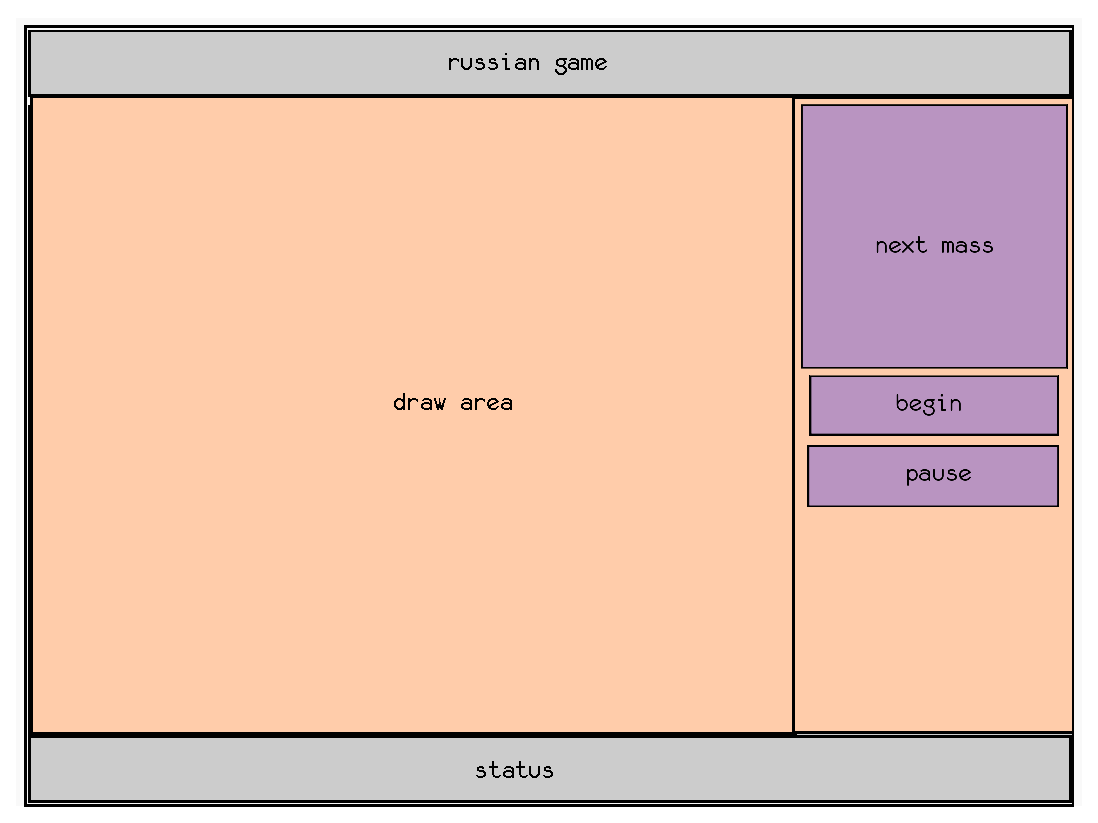
\includegraphics[width=3.5in]{images/interface}
  \caption{程序草图}
  \label{fig:interface}
\end{figure}

``russian game''标题栏和``status''状态栏是GtkLabel控件,``begin''按钮
和``pause''按钮是GtkButton控件,``draw area''(显示区)和``next mass''(下一方
块)是GtkDrawingArea控件。下一个要说明的是控制中部游戏区大小,游戏区由左边``draw
area''(显示区),右边控制区组成;右边控制区大小由其中控件大小决定,剩下的空间全部
分配给左边的显示区,要达到目的,左边显示区需放
入alignment1(GtkAlignment控件)中,右边控制区alignment2(Gtkalignment控
件)中,alignment1的展开属性设为``是'',alignment2的展开属性设
为``否'',见\pageref{fig:align}页图\ref{fig:align}。我们把以下分析用树形结构表示
出来,是这样的:

\begin{shell}
\begin{verbatim}
GtkWindow
  - GtkVBox
     - GtkLabel
     - GtkHBox
     |    - GtkAlignment
     |    |   - GtkDrawingArea
     |    - GtkAlignment
     |       - GtkVBox
     |          - GtkDrawingArea
     |          - GtkButton  
     |          - GtkButton
     - GtkStatusBar
\end{verbatim}
\end{shell}

\begin{figure}[htbp]
  \centering
  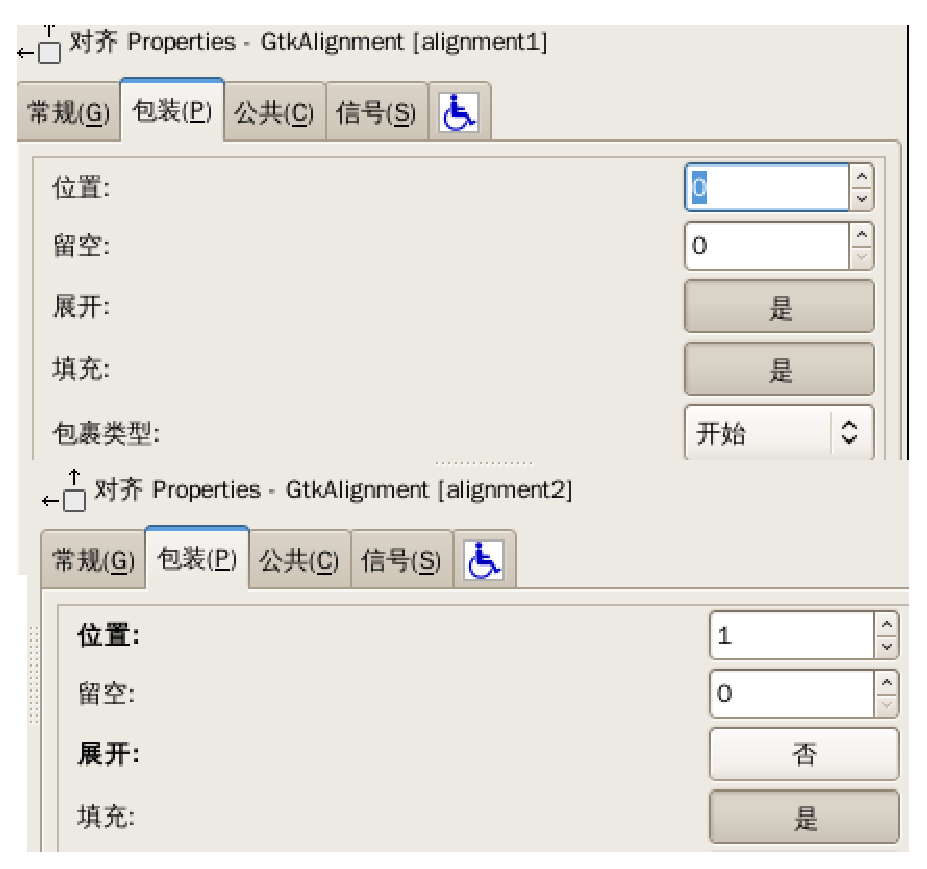
\includegraphics[width=3.5in]{images/align}
  \caption{	设置alignment}
  \label{fig:align}
\end{figure}


\end{document}

